 % !TEX root = report.tex
 % !TEX program = xelatex
 
\subsection{终端命令解析与处理 \texttt{VT100Parser}}

对于终端的命令,我们支持VT220标准\footnote{\url{https://vt100.net/docs/vt220-rm/}}下几乎所有的会影响显示结果的命令,以及XTerm\footnote{\url{http://invisible-island.net/xterm/ctlseqs/ctlseqs.html}}下常用的光标控制以及字符编辑命令,可以支持解析绝大多数程序的输出。目前所支持的命令见表\ref{tab:supported-commands}。

终端具有多种内部状态,例如光标位置、光标是否闪烁和滚动区域等,这些状态均会影响到各个命令的行为。我们的命令处理模块主要维护了表\ref{tab:inner-status}中所列的内部状态。各类状态的具体维护由各个子模块进行处理。

\begin{table}
	\centering
	\begin{tabular}{|l|l|} \hline
		\texttt{cursor.x} & 光标的X坐标 \\ \hline
		\texttt{cursor.y} & 光标的Y坐标 \\ \hline
		\texttt{graphics.bg} & 背景色 \\ \hline
		\texttt{graphics.fg} & 前景色 \\ \hline
		\texttt{graphics.effect} & 表\ref{tab:ram_bytefield}中所列特效 \\ \hline
		\texttt{mode.origin\_mode} & Origin模式 \\ \hline
		\texttt{mode.auto\_wrap} & AutoWrap模式 \\ \hline
		\texttt{mode.insert\_mode} & Insert模式 \\ \hline
		\texttt{mode.line\_feed} & LineFeed模式 \\ \hline
		\texttt{mode.cursor\_blinking} & 光标是否闪烁 \\ \hline
		\texttt{mode.cursor\_visibility} & 光标是否可见 \\ \hline
		\texttt{attrib.scroll\_top} & 滚动区域顶 \\ \hline
		\texttt{attrib.scroll\_bottom} & 滚动区域底 \\ \hline
		\texttt{attrib.charset} & 字符集 \\ \hline
		\texttt{prev\_data} & 上一个输入的字符 \\ \hline
	\end{tabular}
	\caption{终端内部状态表}
	\label{tab:inner-status}
\end{table}

\subsubsection{命令解析模块 \texttt{CommandsParser}}
终端的命令主要的格式是

\begin{center}
	\textit{Introducer Parameters Terminator}
\end{center}

它们表示命令开始、命令参数和命令结束。其中\textit{Introducer}主要是由ESC或CSI\footnote{即ESC [}构成,\textit{Parameters}可以有多个,并且用分号分隔。

命令解析模块主要是将串口收到的字节流解析为对应的命令,并且将参数提供给后续模块的处理。

命令的解析是通过如图\ref{fig:command_parser}所示的状态机来进行实现,主要在\texttt{CommandsParser}模块中。在解析完成一条命令后会产生一个\texttt{commandsReady}信号,并且附带额外的命令参数等信息以供后续模块执行对应操作。

大部分命令的参数个数以及格式均是固定的,解析较为简单。有两类特殊的命令,其参数个数不定,它们分别是控制显示字符的颜色等信息的命令,以及设置/清除终端某些状态的命令。这两类命令的参数均为零或多个由分号分隔的数字构成,参数的个数任意。

对于这两个命令的解析,我们采用另外的方法:

\begin{enumerate}
	\item 当一条命令开始时产生一个\texttt{commandsReady}信号并且对应INIT\_PNS命令,后续需要处理这两类命令的模块在收到此命令时重置其中状态机。
	\item 每当获取到一个参数后产生一个\texttt{commandsReady}信号,并且对应一个EMIT\_PNS的命令,后续需要处理这两类命令的模块在收到此命令后根据所得到的参数在其自身内部的状态机内进行处理(具体的处理方法见各模块的描述)。
	\item 当真正解析到该条命令结尾时,产生对应命令的信号,后续模块将之前所记录的信息应用到终端的状态中更新其状态。
\end{enumerate}

\begin{longtable}{|r|l|l|}
	\caption{当前支持的命令}
\label{tab:supported-commands} \\

\hline
\textbf{命令名称} & \textbf{命令格式} & \textbf{命令行为} \\ \hline
CUU & \texttt{ESC [ Pn\footnote{Pn表示数值参数,可以省略} A} & 光标上移\\ \hline
CUD & \texttt{ESC [ Pn B }& 光标下移\\ \hline
CUF & \texttt{ESC [ Pn C }& 光标前进\\ \hline
CUB & \texttt{ESC [ Pn D }& 光标后退\\ \hline
CNL & \texttt{ESC [ Pn E }& 光标下移到行首\\ \hline
CPL & \texttt{ESC [ Pn F }& 光标上移到行首\\ \hline
CHA & \texttt{ESC [ Pn G }& 光标水平移动\\ \hline
VPA & \texttt{ESC [ Pn d }& 光标垂直移动\\ \hline
CUP/HVP & \texttt{ESC [ Pn; Pn f/H }& 设置光标位置\\ \hline \hline

REP & \texttt{ESC [ Pn b }& 重复上一个输入的字符 \\ \hline
DL & \texttt{ESC [ Pn M }&删除行 \\ \hline
IL & \texttt{ESC [ Pn L }&插入行 \\ \hline
ED &\texttt{ESC [ Pn J }&删除部分显示的文本 \\ \hline
EL &\texttt{ESC [ Pn K }&删除部分当前行文本 \\ \hline
ECH & \texttt{ESC [ Pn X }&清除部分字符 \\ \hline
DCH & \texttt{ESC [ Pn P }&删除部分字符 \\ \hline
ICH & \texttt{ESC [ Pn @ }&插入空白字符 \\ \hline \hline

HTS & \texttt{ESC H }& 设置TabStop \\ \hline
TBC & \texttt{ESC [ Pn g }& 清除TabStop \\ \hline \hline

SETDEC & \texttt{ESC [? Ps\footnote{Ps表示由分号分隔的个数不定的数值参数列} h }& 设置DEC模式 \\ \hline
RESETDEC & \texttt{ESC [? Ps l }& 清除DEC模式 \\ \hline
SETMODE &\texttt{ESC [ Ps h }& 设置模式 \\ \hline
RESETMODE & \texttt{ESC [ Ps l }&清除模式 \\ \hline \hline

NEL & \texttt{ESC E }&新行 \\ \hline
RI & \texttt{ESC M }& 回到上一行 \\ \hline
IND & \texttt{ESC D }&转到下一行 \\ \hline
DECSC & \texttt{ESC 7}& 保存光标状态 \\ \hline
DECRC &\texttt{ESC 8}& 恢复光标状态 \\ \hline \hline

SU & \texttt{ESC [ Pn S }&向上滚动 \\ \hline
SD & \texttt{ESC [ Pn T }&向下滚动 \\ \hline
DECSTBM & \texttt{ESC [ Pn; Pn r }&设置滚动区域 \\ \hline \hline

SS2 & \texttt{ESC N}&设置字符集 \\ \hline
SS3 & \texttt{ESC O}&设置字符集 \\ \hline
SCS0 & \texttt{ESC ( A/B/0/1/2 }& 设置字符集 \\ \hline
SCS1 & \texttt{ESC ) A/B/0/1/2 }&设置字符集 \\ \hline \hline

SGR & \texttt{ESC [ Ps m }&设置颜色等字符信息 \\ \hline
\end{longtable}

本模块中还初始化了下列的子模块。

\subsubsection{光标控制模块 \texttt{CursorControl}}
该模块主要负责控制光标的位置。光标的位置受到多种命令和终端状态的控制:

\begin{itemize}
	\item 当新输入一个字符时,光标右移一格。当光标处于行末时,若处于AutoWrap模式,则跳到下一行的第一个位置,否则不动。
	\item 当输入LF、FF和VT时,光标移动到下一行的同一列。若处于LineFeed模式则还会移动到行首。
	\item 当输入BS时,光标回退一格,若处于行首则不动。
	\item 当输入HT时,移动到下一个TabStop位置。
	\item 当滚动区域改变时,光标移动到原点。
	\item 对于REP命令,光标的行为和插入字符相同。
	\item 对于IL、DL命令,光标移动到行首。
	\item 其余直接控制光标的命令,诸如CUU、CUD、CUF和CUB等。
\end{itemize}

光标的位置的原点取决于是否处于Origin模式。若处于Origin模式,则原点位于滚动区域的原点,否则位于整个屏幕的原点。

对于部分命令,其对光标的操作会出发滚动屏幕的操作。这会引起一个名为\texttt{scrollReady}的信号被设置,并且附带一部分滚动屏幕的参数,交由\texttt{TextControl}模块处理。

对于制表符的处理,当输入这类字符时,该模块不会直接处理,\texttt{TabControl}发现该命令会寻找下一个TabStop的位置,并且在找到后产生一个\texttt{TabReady}信号并且附带查找到的位置。本模块在接受到这样的信号时再将光标设置到对应位置。

\subsubsection{制表符控制模块 \texttt{TabControl}}
该模块主要负责TabStop的设置和光标位置的寻找。默认情况下,每8个字符会有一个TabStop。

当输入一个VT字符后,会引起光标跳转到下一个TabStop的位置。该模块会通过一个状态机进行循环,查找下一个TabStop位置,并且反馈给\texttt{CursorControl}模块设置光标位置。

此外,有TBC和HTS两条命令可以设置不同的TabStop位置,也由该模块进行处理。
\subsubsection{字符控制模块 \texttt{TextControl}}
该模块负责TextRam的读写,用于施加编辑命令产生的改变。控制整个模块功能的状态机如图\ref{fig:text_control}所示。

\begin{figure}[htbp]
\centerline{
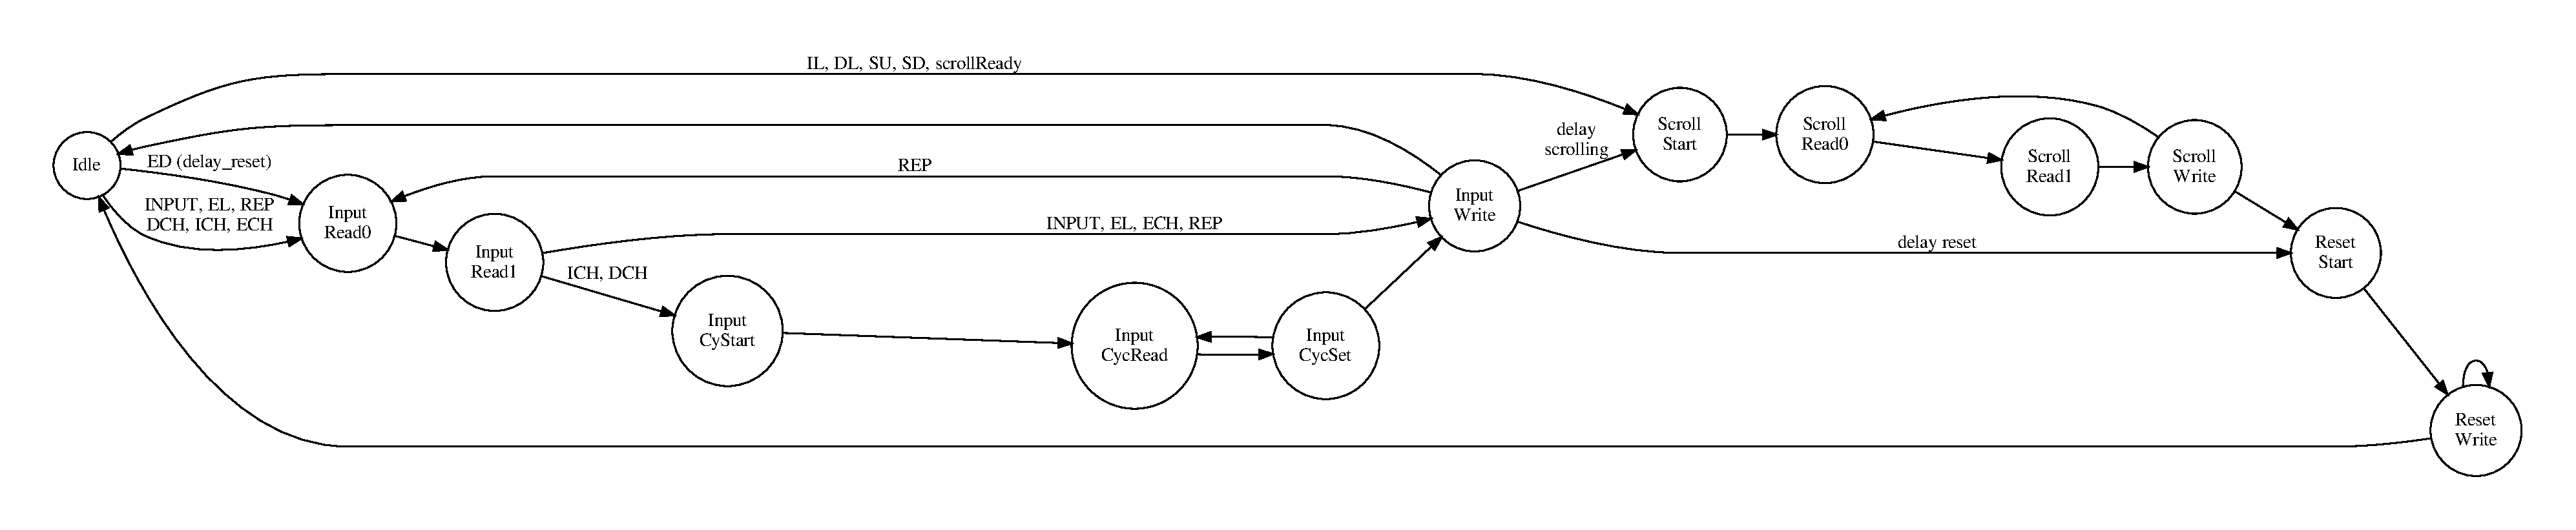
\includegraphics[width=0.95\paperwidth]{text_control.pdf}
}
\caption{字符控制模块状态图。}
\label{fig:text_control}
\end{figure}

该模块对TextRAM的操作主要由三种基本操作组成:

\paragraph{行内编辑}
主要负责对一行内的信息进行编辑,一共分为三种编辑方法,
\begin{enumerate}
	\item 将指定行某个区间的所有字符设置成特定字符(记为A类命令)。
	\item 将指定区间的字符删除,右侧字符左移并且在空白处填充空字符(记为B类命令)。
	\item 在指定区间插入空字符,原有字符右移,若超出屏幕则丢弃(记为B类命令)。
\end{enumerate}

其状态主要为InputRead0、InputRead1、InputCycStart、InputCycRead、InputCycSet、InputWrite组成,它们的意义分别为

\begin{itemize}
	\item \textit{InputRead0.} 发送读请求,读取所需要编辑的行。
	\item \textit{InputRead1.} 等待数据到达。如果是A类命令,则直接用一个组合逻辑进行计算输出值,并且跳转到InputWrite;如果是B类命令,由于组合逻辑过于复杂,跳转到InputCycStart通过时序逻辑来完成。
	\item \textit{InputCycStart.} 将当前行的数据锁存,并且初始化后续需要的变量(当前所编辑的列,当前所需要读取的列)。
	\item \textit{InputCycRead.} 从锁存的行数据中读取当前所需要读取的列对应的字符,并存储。
	\item \textit{InputCycWrite.} 将存储的字符写入当前所编辑的列。并且更新当前列和所需要读取的列。
	\item \textit{InputWrite.} 将编辑完成的行写入。
\end{itemize}

\paragraph{屏幕滚动}
主要负责将某区域上移/下移指定行数。

该部分主要由ScrollStart、ScrollRead0、ScrollRead1和ScrollWrite组成,它们的意义分别为

\begin{itemize}
	\item \textit{ScrollStart.} 设置起始的行。
	\item \textit{ScrollRead0.} 将读请求发送给TextRam。
	\item \textit{ScrollRead1.} 等待数据到达。
	\item \textit{ScrollWrite.} 将数据写入对应行。
\end{itemize}

\paragraph{多行清空}
主要负责将某区域填充为空字符。

该部分主要由ResetStart和ResetWrite两个状态控制。其中ResetStart负责设置起始的行,而后ResetWrite不断往下,每次向RAM中写入一个空行直到所需要清除的区域结束为止回到Idle状态。

该模块所处理的所有命令均可以通过这三种基本操作的组合构成,组合的操作基本有

\paragraph{滚屏}
在``屏幕滚动''结束后跳转到``多行清空'',将因为滚动产生的空位设置为空字符。

\paragraph{插入编辑}
当光标位于行末且处于插入编辑模式,在输入一个字符后会输入一个字符,并且产生一个新行。此种类型优先进行``行内编辑'',并且设置一个\texttt{delay\_scrolling}标记,在行内编辑结束后跳转到``滚屏''。

\paragraph{混合删除}
对于ED命令,会删除光标至屏幕末尾所有的字符,这分为两个步骤。首先是``行内编辑''清除光标所在行的字符,并且设置\texttt{delay\_reset}标记,在行内编辑结束后跳转到``多行清空''再清除剩余的内容。
\paragraph{跨行插入}
对于REP命令,其功能要求是插入指定字符,这可以跨越多行。这类操作会使用``行内编辑'',但同时设置一个\texttt{rep\_mode}标记,同时设置必要的插入到何处的参数。之后``行内编辑''一行结束后检查是否到跨行插入的最后一行,如果不是则继续跳转到``行内编辑''初始处。

对于不同的命令,分别初始化不同的组合操作参数进行处理。
\subsubsection{图形控制模块 \texttt{GraphicsControl}}
该模块主要负责处理字符的颜色和特效(下划线、闪烁、反色和增亮)。对应的命令为SGR,其参数个数不定,且共分为3种类别
\begin{enumerate}
	\item 仅用一个参数表示的属性,这部分对应于VT220的标准。
	\item 需要三个参数表示的属性,这是在一个256色的颜色表中指定对应颜色,其格式为 {\it 48/38; 5; Pn},其中38表示前景色,48表示背景色,Pn表示颜色的编号。
	\item 需要五个参数表示的属性,这是用RGB指定颜色,其格式为 {\it 48/38; 2; R; G; B},其中38表示前景色,48表示背景色。
\end{enumerate}

这条命令可以在一个命令内同时设置多个属性,例如{\it ESC [ 38; 5; 100; 48; 2; 0; 0; 255m}就是设置前景色为编号为100的颜色并且设置背景为蓝色。

	对应的状态机见图\ref{fig:graphics_control},具体操作见``命令解析''中多参数命令的处理方法。
\begin{figure}[htbp]
\centerline{
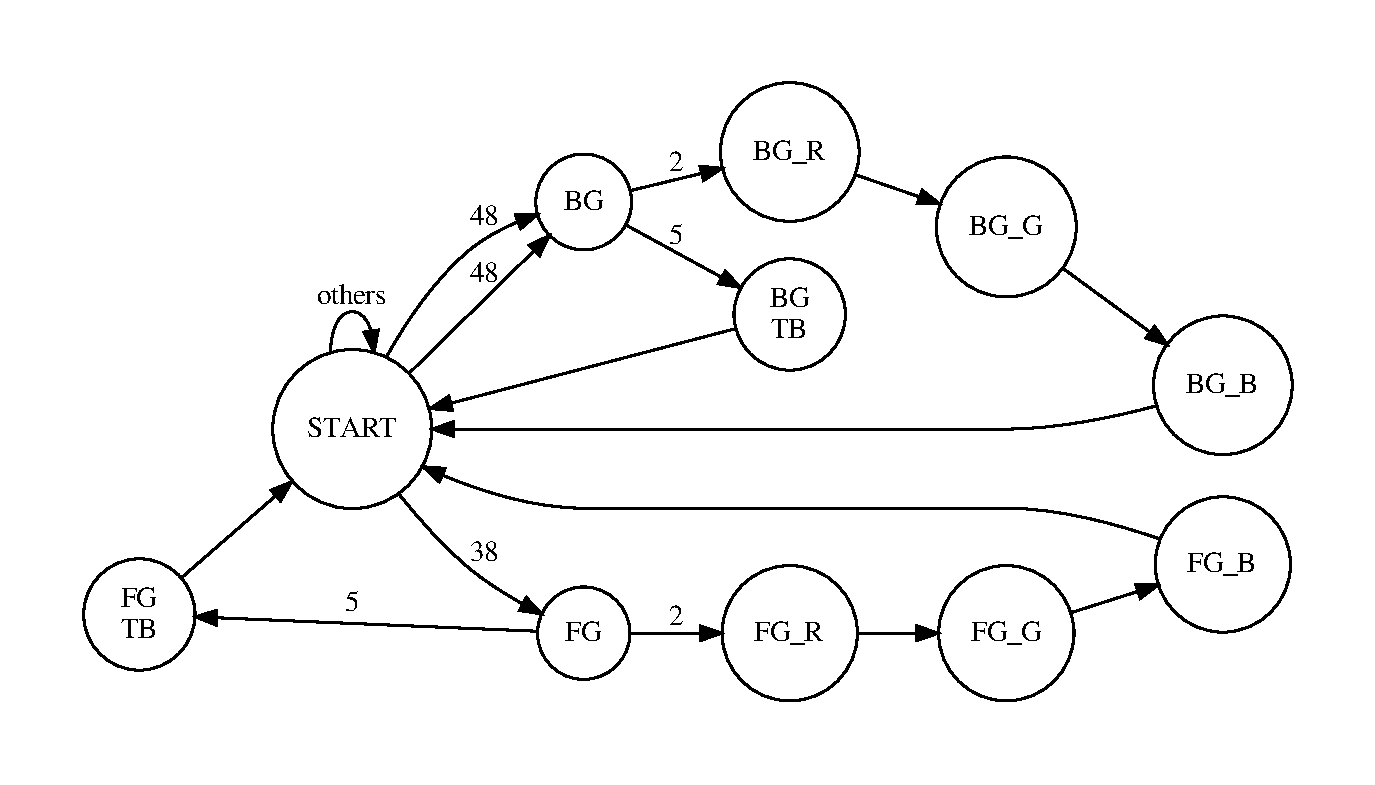
\includegraphics[width=\linewidth]{graphics_control.pdf}
}
\caption{图形控制模块状态图}
\label{fig:graphics_control}
\end{figure}
\subsubsection{属性控制模块 \texttt{AttribControl}}
该模块是对滚动区域、字符集等属性设置命令的处理,较为简单,仅仅在得到命令后直接更新即可。
\subsubsection{模式控制模块 \texttt{ModeControl}}
该模块和图形控制模块同样是一个对应于多参数命令的模块,但是各个属性均可只用一个参数表示,在记录完毕所需要更新的模式后,在更新命令到来时直接更新即可。

\begin{landscape}
	\begin{figure}[htbp]
	\centerline{
	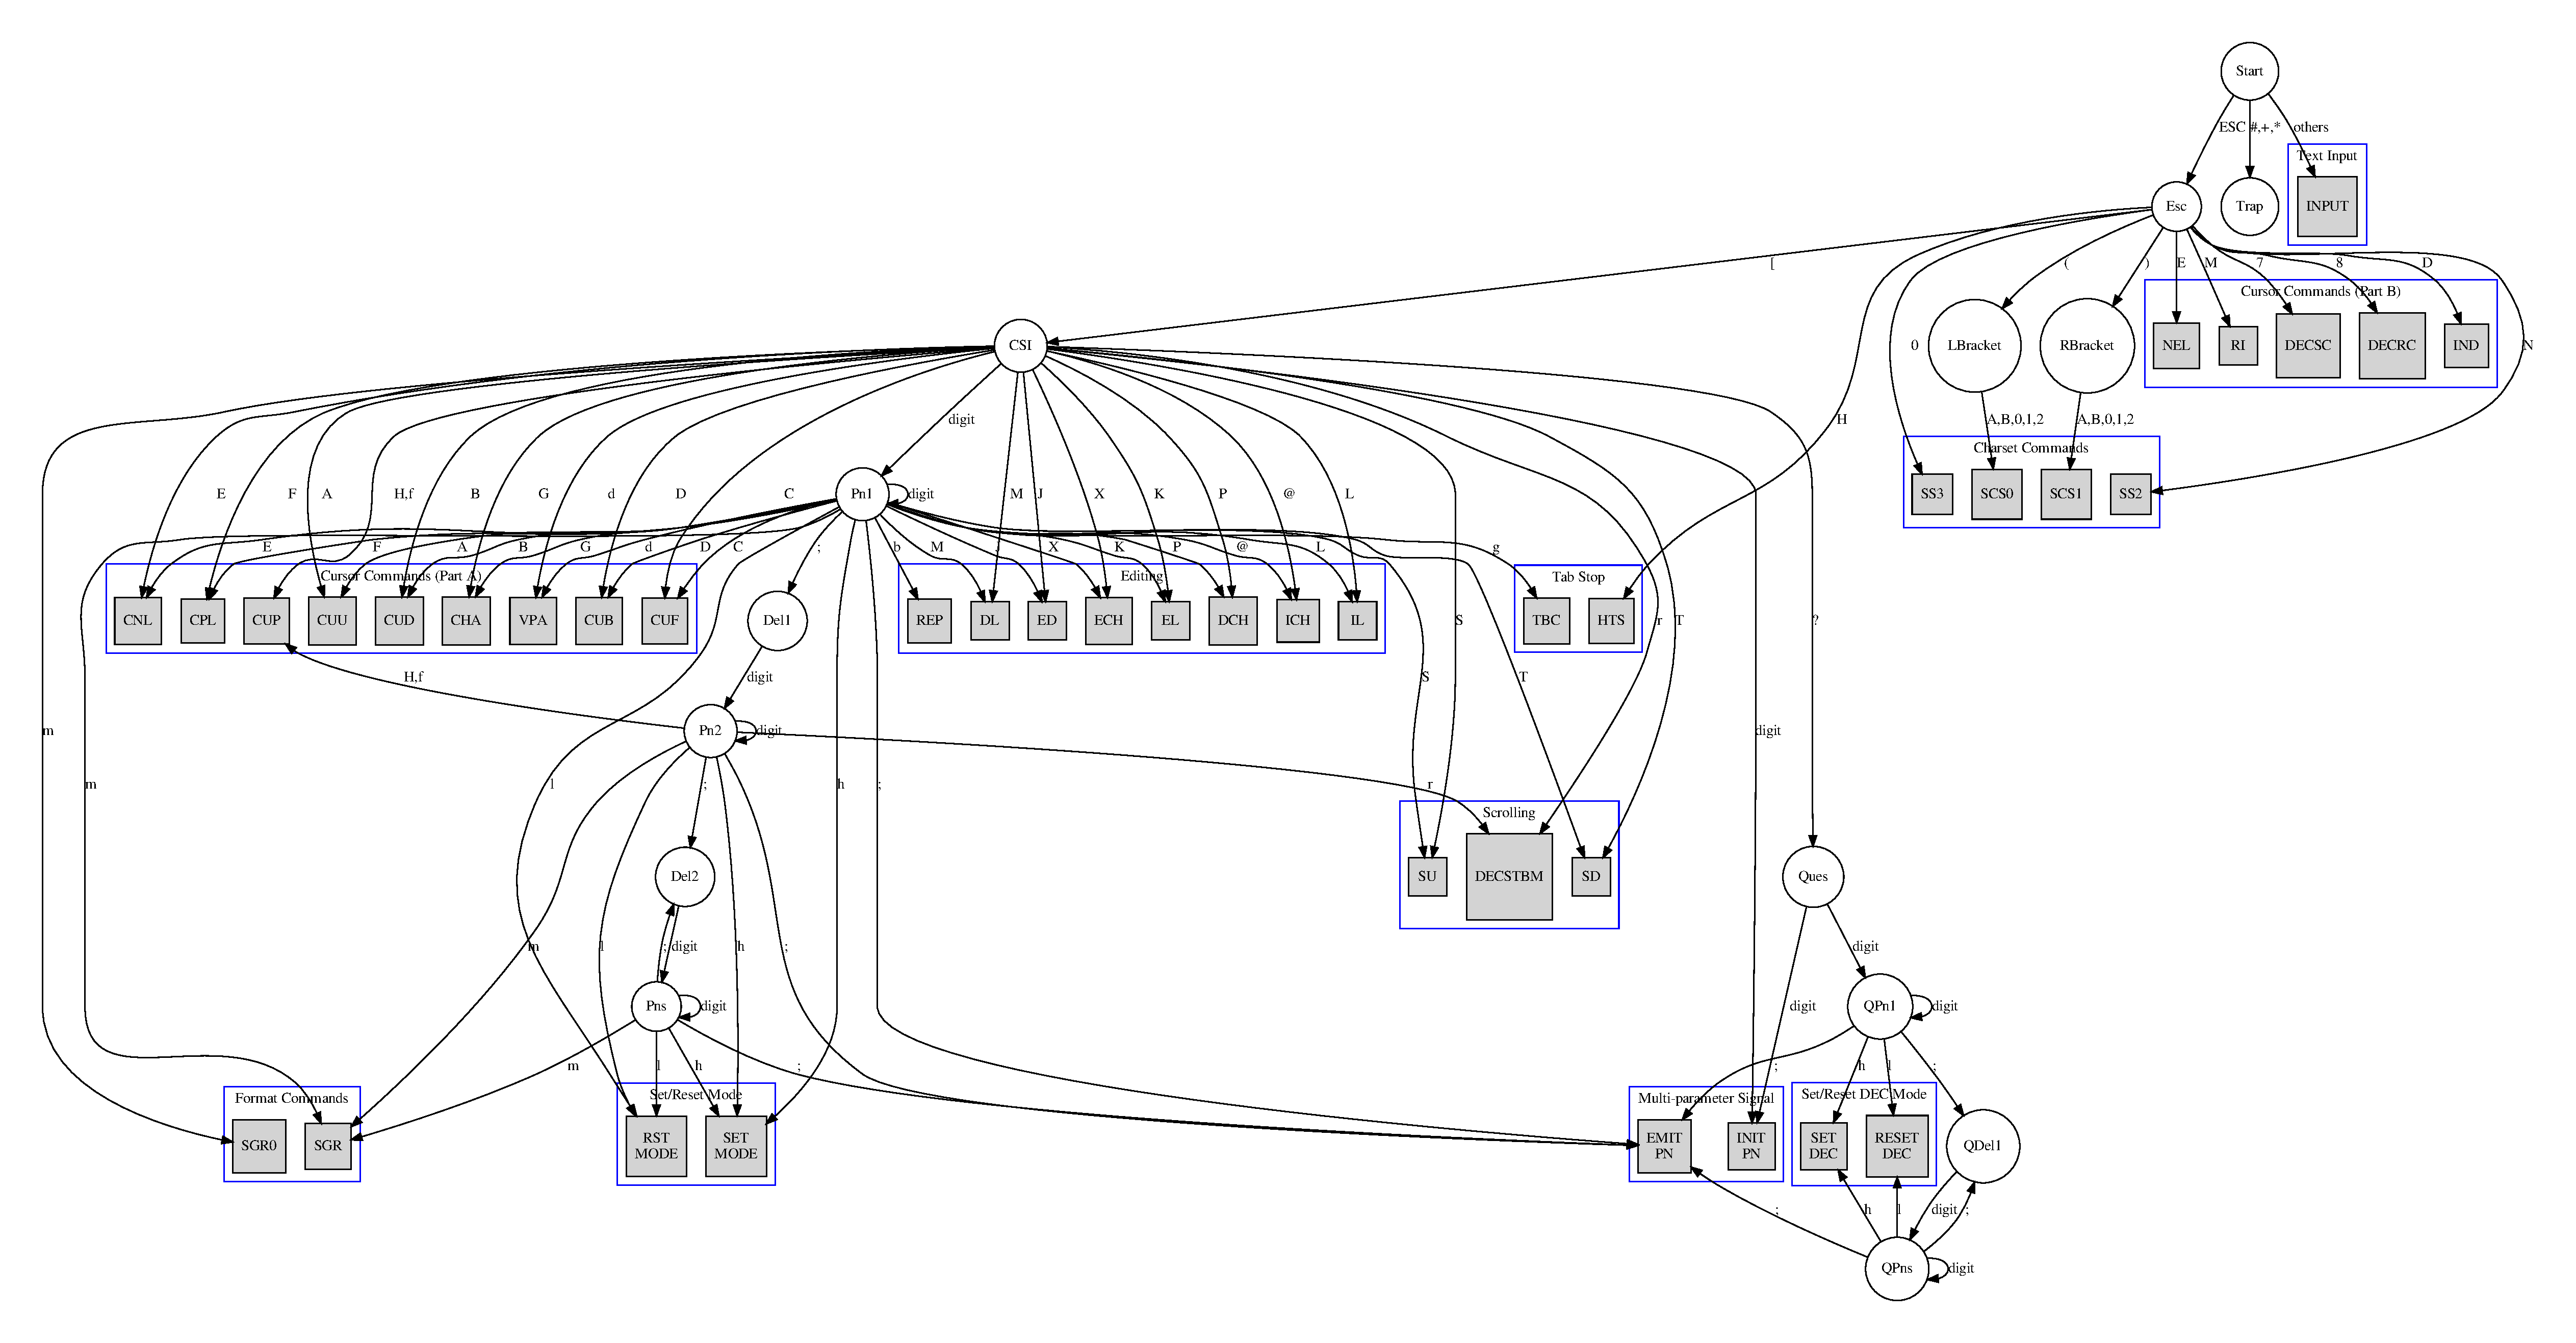
\includegraphics[height=0.95\textheight]{command_parser.pdf}
	}
	\caption{命令解析状态图,圆形节点为状态,方形为命令。}
	\label{fig:command_parser}
	\end{figure}
\end{landscape}
